\subsection{Self-speed Estimator}
\label{sec:self-speed_estimator}
The vehicle's self-speed is used for distinguishing between points of stationary and moving objects and filtering out the points of moving objects in a later block of the pipeline.
It therefore needs to be determined in a reliable way.
Traditional approaches usually utilize external sensors such as wheel encoders, Global Positioning System (GPS), or Inertia Measurement Units (IMUs).
In this project, a technique was developed that determines the vehicle's self-speed only by processing the point cloud's data.
An angle $\phi_{p}$ was defined between each individual point of the point cloud and the radar sensor's centerline:
\par
\begin{figure}[!htbp]
    \centering
    %\resizebox{0.48\textwidth}{!}{
        \begin{tikzpicture}
            \gokart{0}{0}{0}

            \coordinate(O) at (0,0);
            \coordinate(P) at (0.75,1.5);
            \coordinate(A) at (0,1.5);

            \draw[dashed, thick, gray] ($(P)!1.2!(O)$) -- ($(O)!1.2!(P)$);
            \draw[dashed, thick] ($(A)!1.2!(O)$) -- ($(O)!1.24!(A)$);
            \draw pic["$\phi_{p}$", draw=black, angle radius=1.68cm, angle eccentricity=0.85] {angle=P--O--A};
            \draw[fill=red] (P) circle (0.07) node [right] {\small $p$};

            \draw[->, thick, red] (-0.2,0) -- (0.4,0) node[above] {\small $x$};
            \draw[->, thick, red] (0,-0.2) -- (0,0.4) node[left] {\small $y$};
            \fill[red] (0,0) circle (0.05);
        \end{tikzpicture}
    %}
    \caption{Definition of the angle $\phi_{p}$}
    \label{fig:def_angle_phi}
\end{figure}
\FloatBarrier\noindent
These angles $\phi_{p}$ can be calculated using the points' cartesian position information:
\begin{equation*}
    \phi_{p} = arctan\left(\frac{x_{p}}{y_{p}}\right)
    \label{eq:calc_angle_phi}
\end{equation*}
A curve $v(\phi)$ is fitted through the points with their angles $\phi_{p}$ serving as the independent variable and their radial speeds $v_{r,p}$ as the dependent variable.
The curve's value $v(\phi = \SI{0}{\degree})$ then gives an estimation for the vehicle's self speed.
\par
This is possible because the perceived radial speed $v_{r,p}$ of a point related to a stationary target is dependent on the angle $\phi_{p}$ and follows a cosine when being passed at a certain speed $v_{0}$:
\begin{equation*}
    v_{r,p}(v_{0},\phi_{p}) = -v_{0} \cdot cos(\phi_{p})
\end{equation*}
At $\phi = \SI{0}{\degree}$, the radial speed is therefore equal to the vehicle's self speed.
Because there is rarely a point exactly at \SI{0}{\degree} and the radial speeds of the points also include noise, the approach uses all available points after the first filtering stage to fit a curve and effectively give the best possible estimation.
The implementation uses a least squares polynomial regression approach to fit a 2nd order polynomial (see \cite{numpy_polyfit}), which is sufficient in this case as the angle $\phi$ is defined in a way that $\phi_{p} = \left[-\frac{\pi}{2},\frac{\pi}{2}\right]$, so the cosine can be approximated by a 2nd order polynomial:
\begin{equation*}
    cos(\phi_{p}) \approx a \cdot \phi_{p}^2 + b \quad with\enspace \phi_{p} = \left[-\frac{\pi}{2},\frac{\pi}{2}\right]
\end{equation*}
Multiple runs of this algorithm with recorded test data proved the technique's principle.
\begin{figure}[!htbp]
    \centering
    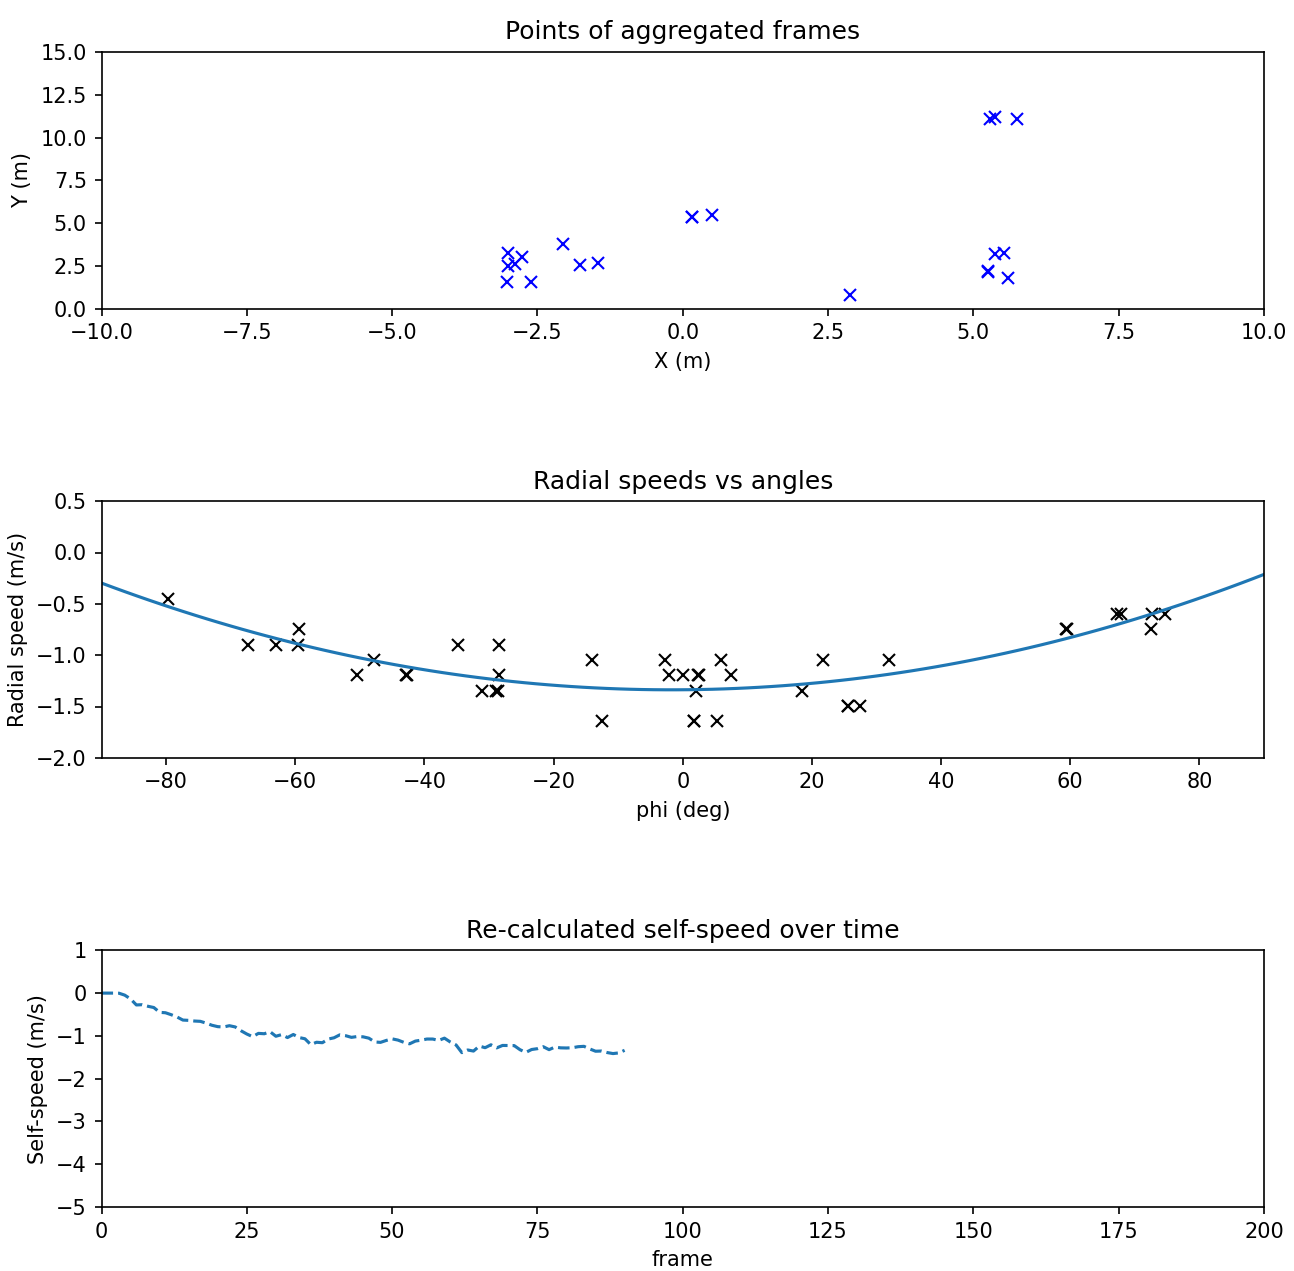
\includegraphics[width=1.0\linewidth]{images/self_speed_reality.png}
    \caption{Test run with recorded data and visualization.}
    \label{fig:self_speed_test_data}
\end{figure}
\FloatBarrier\noindent
During tests, the self-speed estimated by this technique matched the go-kart's built-in speed indicator with some small static offset but also showed heavy fluctuations from time to time when the radar sensor's output only contained a small amount of points.
Although this influence could be reduced by tuning the amount of frames stored in the frame aggregator, a stage containing a Kalman Filter was added after the self-speed estimation before the self-speed value is passed to the following pipeline blocks.



%% [20/03/2025] Leander: Rework done, commentend out bc. probably not needed anymore
%% ---------------------------------------
\begin{comment}

\todo {This whole chapter needs to be done again}
The estimation of a vehicle’s self-speed is a fundamental requirement for autonomous navigation and advanced driver-assistance systems (ADAS). Traditional methods often rely on external sensors such as wheel encoders, GPS, or IMUs to determine vehicle velocity. However, in this project, no external sensor was used for speed estimation. Instead, velocity was estimated exclusively using data from an mmWave radar sensor, leveraging its Doppler measurements to infer motion.

The proposed approach estimates ego-motion (velocity) of the vehicle by analyzing the radial velocity obtained from the radar point cloud. The mmWave radar measures the Doppler shift of each detected point, which corresponds to the relative velocity of objects with respect to the sensor. Assuming that all detected objects are static, the observed Doppler velocities can be directly attributed to the vehicle’s own motion.

\begin{figure}[!htbp]
    \centering
    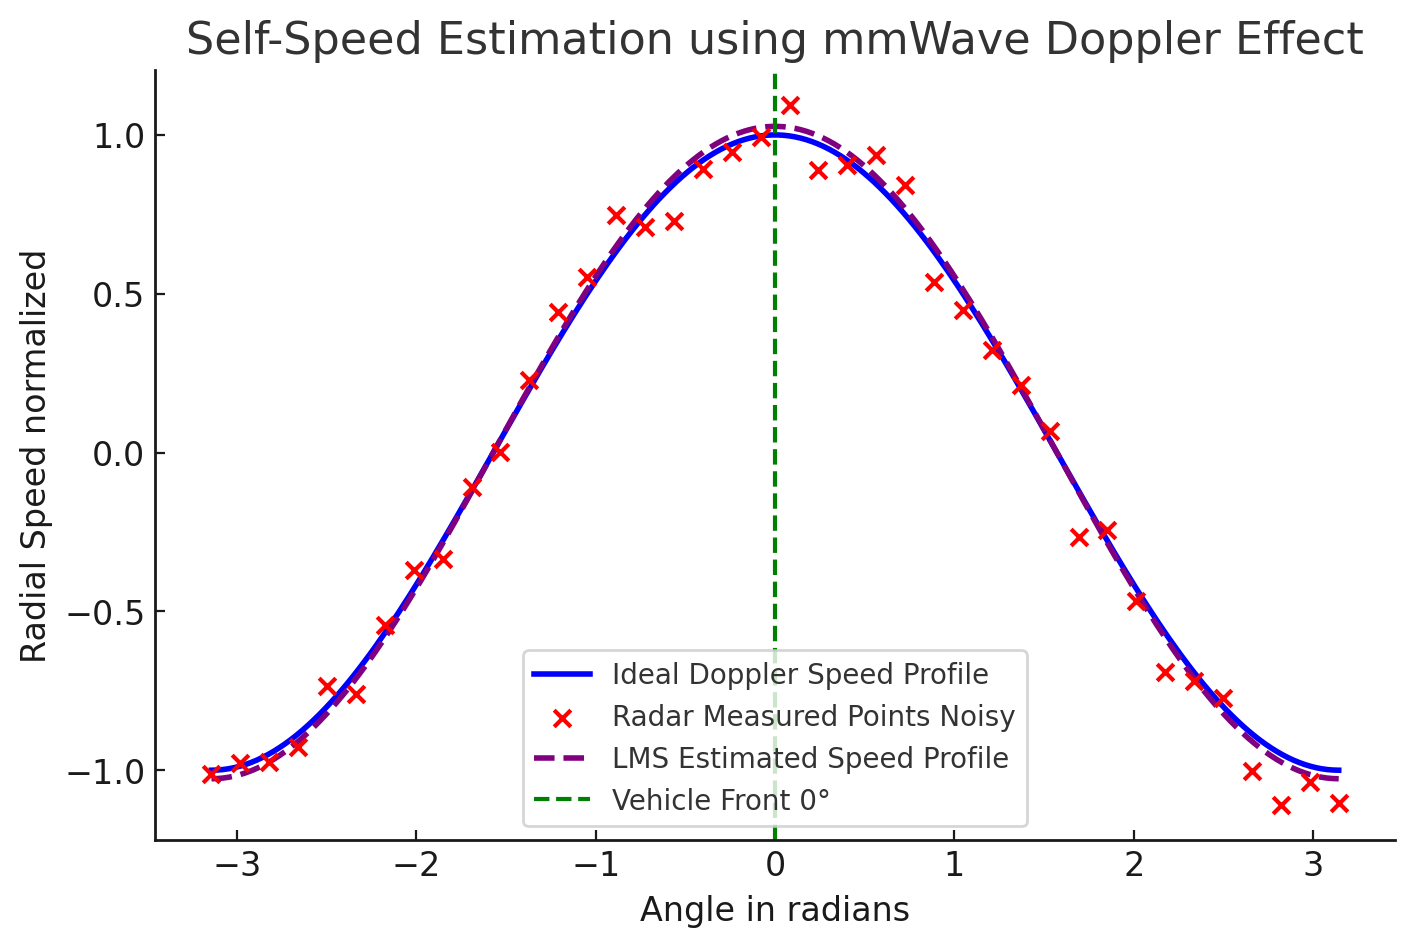
\includegraphics[width=1.0\linewidth]{images/Self_Speed_Doppler.png}
    \caption{Self-Speed Estimation Using MmWave Doppler Effect}
    \label{fig: Self-Speed Estimation Using MmWave Doppler Effect}
\end{figure}
\FloatBarrier\noindent
To estimate speed accurately, radial velocities are fitted to a cosine function that simulates the Doppler shift as a function of detecting angle.  The estimation must be improved, nevertheless, by using an adaptive filtering technique because of measurement noise and differences in detected sites.  The speed estimate is iteratively adjusted in this study by minimizing the error between the measured velocities and the expected cosine profile using the Least Mean Squares (LMS) technique.  This makes it possible to estimate self-speed accurately and reliably without the need for further external sensors.

\subsubsection{Doppler Effect and Speed estimation}

The Doppler effect is a fundamental principle in radar-based velocity estimation. When a vehicle moves, the mmWave sensor measures the radial velocity of detected objects based on the frequency shift of the reflected radar waves. This Doppler shift can be expressed as:

-------------------------------

Estimating the ego-motion (velocity) of a vehicle using radar point clouds can be achieved by analyzing the measured radial velocities (Doppler Shift) from radar returns and solving a least-squares optimization problem. The radar sensor provides radial velocities, which are essentially the component of the actual velocity vector along the radar's line of sight.
However this velocity will shift depending on the angle that it was obtained. For example the most precise velocity is the one that comes from the objects in front of the vehicle, but the ones in the side will have a certain 'error'.

For obtaining this estimations we need:
\begin{itemize}
    \item Input preparation: Each radar detection provides two primary measurements:
    \begin{itemize}
        \item Angle to the target.
        \item Radial speed (Doppler velocity).
    \end{itemize}
    \item Forming the Data Structure: Each radar point is processed individually, computing the angle  (in radians or degrees) and associating it with the measured radial speed. 
    \item Polynomial Regression (Least Squares Fit): To estimate the ego-velocity, the method fits a polynomial (typically first-order for simplicity) to the radial velocities as a function of the angles. 

    \[
    \min_{a,b} \sum_{i} \left( v_{\text{radial}, i} - (a \phi_i + b) \right)^2
    \]


    \item Velocity Estimation: After obtaining coefficients from the polynomial fit, the ego-velocity estimate is derived from evaluating the polynomial at the central angle:
    \FloatBarrier\noindent
    \begin{equation}
        V_{\text{ego}} = b
        \label{eq:velocity_ego_vehicle}
    \end{equation}
    
\end{itemize}

\end{comment}